\documentclass{article}

\usepackage[fleqn]{amsmath} % This package with the fleqn option aligns equations to the left
\setlength{\mathindent}{0pt} % Set indentation from the left margin

\usepackage{amssymb} % Required for math symbols
\usepackage{graphicx} % Required for inserting images
\usepackage{geometry}

\usepackage{float} % Use this package to control float behavior

\usepackage{algorithm}
\usepackage{algpseudocode}

\usepackage[backend=biber, style=authoryear, citestyle=authoryear]{biblatex}
\addbibresource{references.bib}

\geometry{a4paper, margin=1in}

{
\title{
    
\includegraphics[width=0.34\textwidth]{/Users/mlnick/documents/images/tsukuba-logo.png} \\
    \vspace{2mm}
    \textbf{Numerical Simulation} \\
    \vspace{3mm}    
    Project 1 \\
    Simulation of Charged Particle Motion in Electromagnetic Fields
}

\author{Mamanchuk Mykola, SID.202420671}
% \date{\today}
\date{\today}
}

\usepackage{listings}
\usepackage{color}

\definecolor{codegreen}{rgb}{0,0.6,0}
\definecolor{codegray}{rgb}{0.5,0.5,0.5}
\definecolor{codepurple}{rgb}{0.58,0,0.82}
\definecolor{backcolour}{rgb}{0.99,0.99,0.99}

\lstdefinestyle{mystyle}{
    backgroundcolor=\color{backcolour},   
    commentstyle=\color{codegreen},
    keywordstyle=\color{magenta},
    numberstyle=\tiny\color{codegray},
    stringstyle=\color{codepurple},
    basicstyle=\ttfamily\footnotesize,
    breakatwhitespace=false,         
    breaklines=true,                 
    captionpos=b,                    
    keepspaces=true,                 
    numbers=left,                    
    numbersep=5pt,                  
    showspaces=false,                
    showstringspaces=false,
    showtabs=false,                  
    tabsize=2
}
\lstset{style=mystyle}

\begin{document}

\maketitle

\section{Introduction}
Project 1 involves the numerical simulation of the trajectory of a charged particle under the influence of electric and magnetic fields using the Boris algorithm. This method is pivotal for accurate simulation in plasma physics, allowing the study of particle behavior in high energy environments like those found in fusion reactors and astrophysical phenomena.

\section{Theoretical Background}
The motion of charged particles in electromagnetic fields is governed by the Lorentz force, which the Boris algorithm effectively models by discretizing the particle's motion into small time steps. The algorithm ensures stability and accuracy, preserving the phase volume and energy to a high degree, which is critical for long-term simulations.

The Boris algorithm is split into several steps:
\begin{itemize}
    \item \textbf{Initial Half-Step:} The velocity is first updated for half a time step using only the electric field.
    \item \textbf{Rotation Step:} The velocity vector is then rotated using a magnetic field-dependent rotation matrix.
    \item \textbf{Final Half-Step:} Another half-step update using the electric field completes the full time step velocity update.
\end{itemize}

These steps are cyclically repeated for each time step to trace the particle's trajectory over time.

\section{Problem Statement}
Given initial conditions of position and velocity, along with constant electric and magnetic fields, compute the trajectory of the particle using the Boris algorithm. The specific tasks involve:
\begin{enumerate}
    \item Demonstrating that the rotation step in the algorithm conserves the magnitude of velocity, hence showing it is a true rotation.
    \item Computing the trajectory over multiple time steps and visualizing the path in a three-dimensional space to observe characteristics such as gyration due to the magnetic field.
\end{enumerate}

\subsection{Preservation of Velocity Magnitude}

The Boris algorithm, widely used in computational physics for simulating the motion of charged particles in magnetic fields, includes a crucial rotation step that is theoretically designed to only alter the direction of the velocity vector without changing its magnitude. This characteristic is essential for accurately capturing the physics of particle motion in a magnetic field without introducing numerical artifacts such as artificial energy gain or loss.

In the rotation step, the velocity vector $\vec{v}^-$ is first updated to $\vec{v}'$ by adding a cross product of $\vec{v}^-$ and a vector $\vec{t}$, which is derived from the magnetic field $\vec{B}$ and the timestep $\Delta t$. The updated velocity $\vec{v}'$ is then used to compute $\vec{v}^+$, involving another cross product with a vector $\vec{s}$. The vector $\vec{s}$ is calculated to ensure that the rotation does not change the magnitude of the velocity vector.

Given the initial velocity $\vec{v}^-$ and magnetic field $\vec{B}$, the vectors $\vec{t}$ and $\vec{s}$ are computed as follows:
\[
\vec{t} = \frac{q \vec{B} \Delta t}{2m}, \quad \vec{s} = \frac{2 \vec{t}}{1 + \vec{t} \cdot \vec{t}}
\]
where $q/m$ represents the charge-to-mass ratio of the particle. The final velocity after the rotation step $\vec{v}^+$ is obtained by:
\[
\vec{v}' = \vec{v}^- + \vec{v}^- \times \vec{t}, \quad \vec{v}^+ = \vec{v}^- + \vec{v}' \times \vec{s}
\]
To demonstrate that this operation preserves the magnitude, we compute the magnitudes of $\vec{v}^-$ and $\vec{v}^+$ before and after the rotation:
\[
\|\vec{v}^-\|, \quad \|\vec{v}^+\|
\]
The preservation of the magnitude can be numerically verified by ensuring that $\|\vec{v}^-\| = \|\vec{v}^+\|$ within numerical precision.
\vspace{3mm}

\textbf{Implementation} follows below:

\begin{lstlisting}[language=python]
import numpy as np

# Constants
qm = 100  # Charge to mass ratio (q/m)
dt = 0.01  # Time step

# Initial conditions
v_minus = np.array([2.0, 3.0, 4.0])
B = np.array([5.0, 7.0, 8.0])

# Compute t and s vectors for Boris algorithm
t = qm * B * dt / 2
s = 2 * t / (1 + np.dot(t, t))

# Boris algorithm to find v_plus
v_prime = v_minus + np.cross(v_minus, t)
v_plus = v_minus + np.cross(v_prime, s)

# Compare magnitudes
magnitude_v_minus = np.linalg.norm(v_minus)
magnitude_v_plus = np.linalg.norm(v_plus)

print("Magnitude of v_minus:", magnitude_v_minus)
print("Magnitude of v_plus:", magnitude_v_plus)
\end{lstlisting}

\begin{figure}[H] % The [H] forces the figure to appear exactly where it is placed in the text
    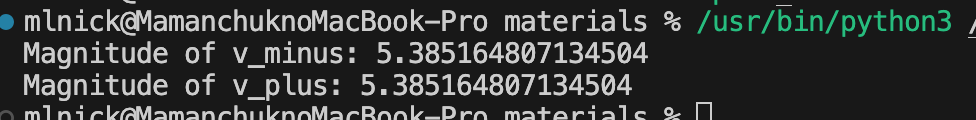
\includegraphics[trim=0 0 0 0, clip, width=0.65\textwidth]{materials/result_1.png} % Adjust trim values to remove padding if necessary
    \label{fig:normal}
\end{figure}


\section{Numerical Implementation}
A Python script utilizing NumPy and Matplotlib is employed for the implementation. The detailed pseudocode is given, followed by the actual Python code used for the simulation.

\subsection{Pesudocode Showcase}

\begin{algorithm}
    \caption{Boris Algorithm for Particle Motion Simulation}
    \begin{algorithmic}[1]
    \State \textbf{Initialize} time step $\Delta t = 0.5 \times 10^{-3}$
    \State \textbf{Initialize} charge-to-mass ratio $qm = 100$
    \State \textbf{Initialize} number of iterations $n_{\text{iter}} = 1000$
    \State \textbf{Initialize} initial velocity $\mathbf{v} = \begin{bmatrix} 2 & 3 & 4 \end{bmatrix}$
    \State \textbf{Initialize} initial position $\mathbf{x} = \begin{bmatrix} 10 & 12 & 1 \end{bmatrix}$
    \State \textbf{Initialize} magnetic field $\mathbf{B} = \begin{bmatrix} 5 & 7 & 8 \end{bmatrix}$
    \State \textbf{Initialize} electric field $\mathbf{E} = \begin{bmatrix} 1 & 2 & 1 \end{bmatrix}$
    \State \textbf{Initialize} memory for positions $\mathbf{x}_{\text{mem}} = \text{zeros}(n_{\text{iter}}, 3)$
    \State \textbf{Calculate} $\mathbf{t} = qm \cdot \mathbf{B} \cdot \frac{\Delta t}{2}$
    \State \textbf{Calculate} $\mathbf{s} = \frac{2 \cdot \mathbf{t}}{1 + \text{dot}(\mathbf{t}, \mathbf{t})}$
    
    \For{$idx = 1$ to $n_{\text{iter}}$}
        \State $\mathbf{v}_{-} = \mathbf{v} + \mathbf{E} \cdot qm \cdot \frac{\Delta t}{2}$
        \State $\mathbf{v}' = \mathbf{v}_{-} + \text{cross}(\mathbf{v}_{-}, \mathbf{t})$
        \State $\mathbf{v}_{+} = \mathbf{v}_{-} + \text{cross}(\mathbf{v}', \mathbf{s})$
        \State $\mathbf{v} = \mathbf{v}_{+} + \mathbf{E} \cdot qm \cdot \frac{\Delta t}{2}$
        \State $\mathbf{x} = \mathbf{x} + \frac{\mathbf{v}_{+} + \mathbf{v}_{-}}{2} \cdot \Delta t$
        \State $\mathbf{x}_{\text{mem}}[idx, :] = \mathbf{x}$
    \EndFor
    
    \State \textbf{Plot} trajectory in 3D
    \end{algorithmic}
\end{algorithm}

\subsection{Python Implementation Listing}

\begin{lstlisting}[language=python, title=Implementation of Boris Algorithm for Particle Motion]
import numpy as np
import matplotlib.pyplot as plt

# Initialization
dt = 0.5e-3  # Time step
qm = 100  # Charge-to-mass ratio
n_iter = 1000  # Number of iterations
initial_v = np.array([2., 3., 4.])  # Initial velocity
initial_x = np.array([10., 12., 1.])  # Initial position
b_field = np.array([5., 7., 8.])  # Magnetic field
e_field = np.array([1., 2., 1.])  # Electric field
x_mem = np.zeros((n_iter, 3))  # Memory for positions

# Calculate s and t vectors
t_vec = qm * b_field * dt / 2  # Magnetic field term for velocity rotation
s_vec = 2 * t_vec / (1 + np.dot(t_vec, t_vec))  # Scaling factor for the rotation

# Boris' algorithm
v = initial_v.copy()
x = initial_x.copy()
for idx in range(n_iter):
    # Step 3: Half-step velocity update for electric field
    v_minus = v + (e_field * qm * dt / 2)

    # Step 4: Rotation due to magnetic field
    v_prime = v_minus + np.cross(v_minus, t_vec)
    v_plus = v_minus + np.cross(v_prime, s_vec)

    # Step 5: Complete the velocity step with the second half-step for electric field
    v = v_plus + (e_field * qm * dt / 2)

    # Step 6: Update position, using the average velocity over the timestep
    x += (v_plus + v_minus) / 2 * dt

    # Store the results in x_mem for plotting
    x_mem[idx, :] = x

# Plotting
fig, ax = plt.subplots(subplot_kw={'projection': '3d'}, figsize=(8, 6))
ax.set_xlabel('X')
ax.set_ylabel('Y')
ax.set_zlabel('Z')
ax.plot(x_mem[:, 0], x_mem[:, 1], x_mem[:, 2], label='Particle Trajectory')
ax.legend()
plt.show()
\end{lstlisting}

\section{Results and Discussion}

The results of the numerical simulation of a charged particle's trajectory in a magnetic and electric field are depicted in Figures \ref{fig:normal} and \ref{fig:magnified}. The simulation employs the Boris algorithm, accounting for both electric and magnetic influences on the particle as it progresses through discrete time steps.

\begin{figure}[H] % The [H] forces the figure to appear exactly where it is placed in the text
    \centering
    \fbox{% Add a frame around the image
    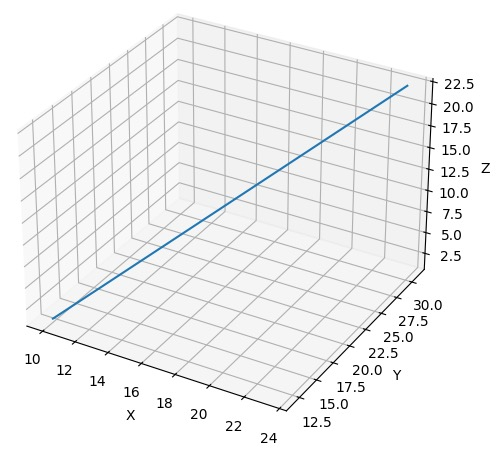
\includegraphics[trim=0 0 0 0, clip, width=0.65\textwidth]{materials/Figure_1.1.jpeg} % Adjust trim values to remove padding if necessary
    }
    \caption{Trajectory of the particle with normal view, illustrating the challenge in observing rotational behavior due to the initial conditions and velocity.}
    \label{fig:normal}
\end{figure}

In Figure \ref{fig:normal}, the trajectory appears as a nearly straight line due to the visualization scale and the relative magnitude of the velocity components. The effect of the magnetic field is subtle under these visualization parameters, highlighting the importance of appropriate scaling in numerical simulations to observe physical phenomena accurately.

\begin{figure}[H]
    \centering
    \fbox{ % Add a frame around the image
    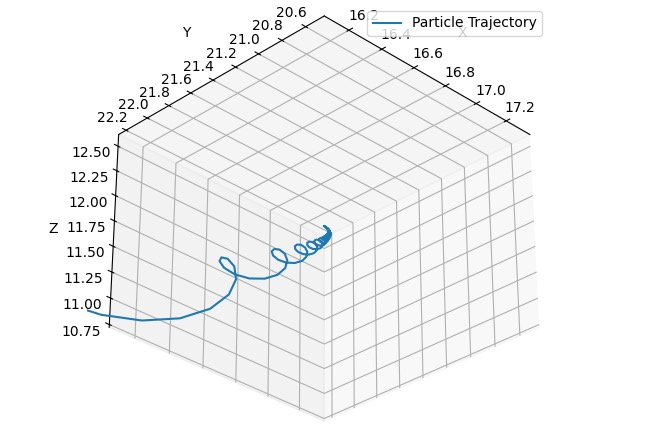
\includegraphics[trim=0 0 0 0, clip, width=0.65\textwidth]{materials/Figure_1.2.jpeg} % Adjust trim values to remove padding if necessary
    }
    \caption{Magnified view of the particle trajectory showing clear rotational motion, which confirms the correct implementation of the Boris algorithm and the impact of the Lorentz force.}
    \label{fig:magnified}
\end{figure}

Figure \ref{fig:magnified} offers a magnified view, revealing the helical nature of the trajectory due to the Lorentz force exerted by the magnetic field. This visualization substantiates the theoretical predictions and demonstrates the rotational dynamics induced by the magnetic interaction. The discrepancy between the two figures emphasizes the need for careful consideration of visualization scales when interpreting simulation results in computational physics.

These findings illustrate the significant impact that initial conditions, scale of visualization, and numerical resolution have on the interpretation of particle dynamics in electromagnetic fields. They underscore the importance of detailed analysis and appropriate graphical representation in studying complex physical systems through computational methods.

\section{Conclusion}
The project concludes with an evaluation of the simulation's effectiveness in modeling particle dynamics in electromagnetic fields and potential improvements or applications of the Boris algorithm in other computational physics projects.


\section*{References}
\begin{enumerate}
    \item \textbf{Mamanchuk N., University of Tsukuba}, Github, \today. Available online: \url{https://github.com/RIFLE}
    % \item \textbf{Company}, Name of Work, year. Available online: \url{https://...} [Accessed: yyyy-mm-dd]
\end{enumerate}

\end{document}
